% =====================================================================
% Ihara--Bass (versión española), companion del lado Ihara a "De signos
% aleatorios a emparejamientos" (Godsil--Gutman, Paper I) y "Desplegar un grafo
% en un árbol" (Heilmann--Lieb, Paper II). Mismo estilo: técnico, no ambiguo,
% narrativo (cada sección abre con una pregunta), fórmulas clave enmarcadas y
% centradas, humildad. Honestidad: "demostrado" = sin sorry; alcance exacto.
% =====================================================================
\documentclass[11pt]{article}
\usepackage[T1]{fontenc}
\usepackage[utf8]{inputenc}
\usepackage{lmodern}
\usepackage[spanish,es-noquoting]{babel}
\usepackage{amsmath,amssymb,amsthm,booktabs,graphicx,hyperref}
\usepackage{xurl}
\usepackage[table]{xcolor}
\definecolor{ggteal}{HTML}{1B6F8C}
\definecolor{ggband}{HTML}{DCE7EB}
\definecolor{ggamber}{HTML}{E08A1E}
\usepackage[margin=1in]{geometry}
\usepackage{microtype}
\usepackage[most]{tcolorbox}
\setlength{\emergencystretch}{6em}
\graphicspath{{figures/}}
\newtheorem{theorem}{Teorema}
\newtheorem{lemma}{Lema}
\newtheorem{definition}{Definici\'on}
\newcommand{\lean}[1]{\texttt{#1}}
\newcommand{\Z}{\mathbb{Z}}
\newcommand{\R}{\mathbb{R}}
\DeclareMathOperator{\Dart}{Dart}
\hypersetup{colorlinks=true,linkcolor=ggteal,citecolor=ggteal,urlcolor=ggteal}
\newtcbox{\keybox}{on line,boxrule=0.9pt,colframe=ggteal,colback=ggband!40,
  arc=3pt,left=8pt,right=8pt,top=5pt,bottom=5pt}
\newcommand{\keyeq}[1]{\begin{center}\keybox{$\displaystyle #1$}\end{center}}

\title{\bf Plegar las aristas en los v\'ertices\\[4pt]
  \large\normalfont Una demostraci\'on verificada por m\'aquina de la f\'ormula del determinante de Bass para la zeta de Ihara en Lean~4}
\author{Carles Mar\'in\thanks{Formalizado con asistencia de IA (Claude, Anthropic); la matem\'atica y todas las afirmaciones son responsabilidad del autor. La metodolog\'ia se discute en la Secci\'on~\ref{sec:implications}.}\\[3pt]
  \normalsize Investigador independiente\\
  \normalsize \texttt{karlesmarin@gmail.com}}
\date{Junio de 2026}

\begin{document}
\maketitle

\begin{abstract}
Este es un trabajo complementario de \emph{De signos aleatorios a emparejamientos}~\cite{PartI} y
\emph{Desplegar un grafo en un \'arbol}~\cite{PartII}, donde formalic\'e el polinomio de
emparejamientos de un grafo---el lado \emph{\'arbol} de un conteo de caminos. Aqu\'i construyo el
lado \emph{ciclo}: una demostraci\'on verificada por m\'aquina, \lean{sorry}-libre, en Lean~4 /
Mathlib, de la \emph{f\'ormula del determinante de Bass} para la funci\'on zeta de Ihara. El
rec\'iproco de la funci\'on zeta es $\det(I-uB)$, donde $B$ es el operador \emph{no-retroceso} de
Hashimoto sobre las $2|E|$ aristas orientadas; el teorema de Bass colapsa ese determinante de
dimensi\'on $2|E|$ a uno de dimensi\'on $|V|$ construido con las matrices de adyacencia y de grados.
Por el camino formalizo el operador no-retroceso, el c\'alculo de incidencia de aristas orientadas y
el determinante $\det(I+uJ)=(1-u^2)^{|E|}$ de la involuci\'on de inversi\'on, para ninguno de los
cuales pude encontrar formalizaci\'on previa en ning\'un asistente de pruebas. El teorema principal
depende solo de los tres axiomas est\'andar. Soy exacto sobre la frontera: demuestro la identidad
\emph{sobre un cuerpo} (el contexto est\'andar; la demostraci\'on invierte $I+uJ$, una unidad
exactamente cuando $1-u^2\neq0$), la funci\'on zeta anal\'itica---el producto de Euler sobre ciclos
primos---\emph{no} est\'a formalizada, y la generalidad sobre anillos arbitrarios queda mapeada, no
construida. Nada de esto es matem\'atica nueva; la contribuci\'on es la formalizaci\'on, y el hecho
de que el lado ciclo de la f\'ormula de traza emparejamientos/Ihara conviva ahora con el lado
\'arbol en la misma biblioteca.
\end{abstract}

\noindent\emph{Mapa para el lector.} Si lees una sola cosa, lee el Teorema~\ref{thm:bass} y la
Figura~\ref{fig:nb}---la identidad, y la imagen de por qu\'e un determinante del tama\~no de las
aristas es en realidad del tama\~no de los v\'ertices. La demostraci\'on es un solo viaje: un c\'alculo de incidencia de
cuatro identidades (Secci\'on~\ref{sec:proof}), el determinante de la involuci\'on de inversi\'on
$\det(I+uJ)=(1-u^2)^{|E|}$ obtenido orientando las aristas (Figura~\ref{fig:reindex}), y un paso de
Sylvester que factoriza $I+uJ$ y desliza las matrices de incidencia una sobre otra. Las f\'ormulas
que sostienen el argumento van enmarcadas; los l\'imites honestos---ante todo la hip\'otesis de
cuerpo---se enuncian con la misma claridad que el resultado.

% ---------------------------------------------------------------
\section{Introducci\'on: una breve historia, y por qu\'e este art\'iculo}
\label{sec:intro}

\emph{¿Podr\'ia una funci\'on zeta nacida en 1966 en la aritm\'etica de grupos $p$-\'adicos,
redescubierta calladamente como un enunciado sobre grafos, y convertida en los a\~nos 2010 en una
herramienta de la ciencia de redes, quedar fuera de toda duda gracias a una m\'aquina---y para qu\'e
servir\'ia?} Responderla exige que se encuentren varios hilos de historia.

El primer hilo es la \emph{teor\'ia de n\'umeros}. En 1966 Ihara~\cite{Ihara1966} asoci\'o una
funci\'on zeta a un subgrupo discreto de $\mathrm{PGL}_2$ sobre un cuerpo $p$-\'adico, como an\'alogo
sin grafos de la funci\'on zeta de Selberg. Serre observ\'o que el objeto de Ihara era en secreto
combinatorio: el grupo $p$-\'adico act\'ua sobre un \'arbol---su \'arbol de Bruhat--Tits---y la zeta
depende solo del \emph{grafo} cociente finito. Despojada de sus or\'igenes aritm\'eticos, la
\emph{funci\'on zeta de Ihara} de un grafo finito $G$ cuenta sus \emph{ciclos primos}---clases de
caminos cerrados que nunca retroceden y no son potencias de otros m\'as cortos---mediante un
producto de Euler $\zeta_G(u)=\prod_{[C]}(1-u^{\ell(C)})^{-1}$. Un teorema de teor\'ia de n\'umeros se
hab\'ia vuelto un teorema de grafos (Figura~\ref{fig:prime}).

\begin{figure}[t]
  \centering
  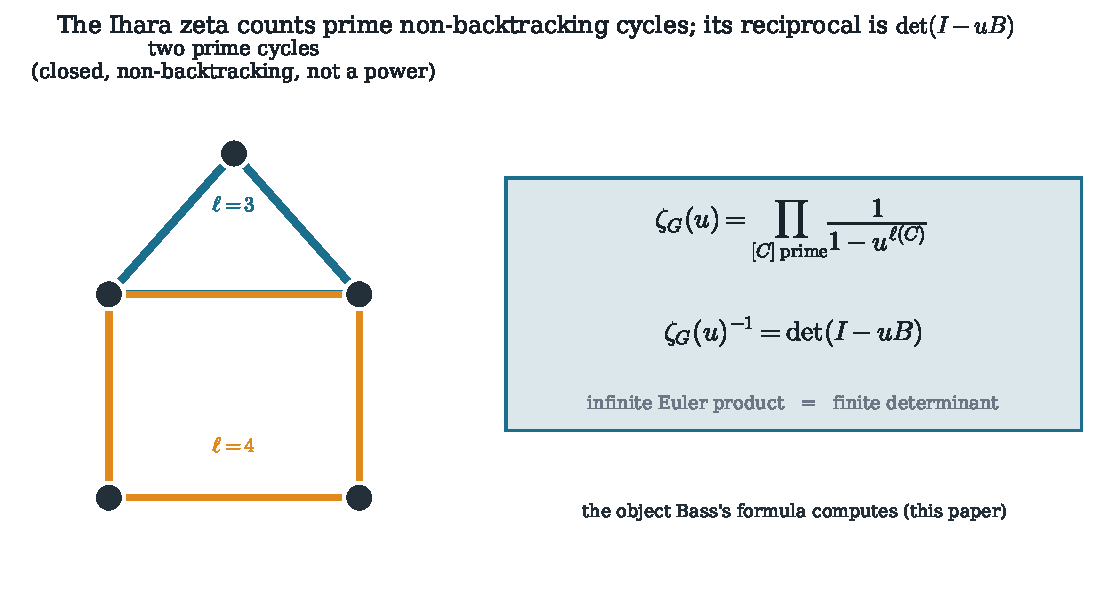
\includegraphics[width=\textwidth]{bass_fig4_primecycles.pdf}
  \caption{Qu\'e cuenta la zeta de Ihara. Los \emph{ciclos primos} de un grafo son sus caminos
  cerrados, no-retroceso, que no son potencias de otros m\'as cortos (se muestran dos, de longitudes
  $3$ y $4$). La zeta es su producto de Euler; su rec\'iproco es el determinante finito
  $\det(I-uB)$---el objeto que computa la f\'ormula de Bass, y que este art\'iculo formaliza.}
  \label{fig:prime}
\end{figure}

El segundo hilo es la \emph{teor\'ia de grafos}. Sunada y luego Hashimoto~\cite{Hashimoto1989}
reformularon la zeta mediante un operador lineal: el operador \emph{no-retroceso} (de adyacencia de
aristas) $B$ sobre las $2|E|$ aristas orientadas, con $\zeta_G(u)^{-1}=\det(I-uB)$. Es un
determinante honesto, pero grande---su tama\~no es el doble del n\'umero de aristas. En 1992
Bass~\cite{Bass1992} demostr\'o la identidad que lo domestica, colapsando el determinante de
dimensi\'on $2|E|$ sobre aristas a uno de dimensi\'on $|V|$ sobre v\'ertices; Kotani--Sunada y
Foata--Zeilberger dieron despu\'es demostraciones elementales~\cite{KotaniSunada2000}, y el
\emph{Stroll through the Garden} de Terras~\cite{Terras2011} es el relato moderno. La f\'ormula de
Bass es el puente entre el operador combinatorio $B$ y los datos espectrales $(A,D)$ que el grafo ya
lleva puestos.

El tercer hilo ata esto a la banda de los art\'iculos anteriores. Un grafo $d$-regular es
\emph{Ramanujan}---un expansor \'optimo, su espectro no trivial dentro de
$[-2\sqrt{d-1},2\sqrt{d-1}]$---precisamente cuando su zeta de Ihara satisface un an\'alogo de la
\emph{hip\'otesis de Riemann} (Sunada): los polos de la zeta caen sobre una recta cr\'itica, imagen
multiplicativa de la misma banda $2\sqrt{d-1}$ que confina las ra\'ices del polinomio de
emparejamientos en \emph{Desplegar un grafo en un \'arbol}~\cite{PartII}. El polinomio de
emparejamientos es la sombra \'arbol (Plancherel) del conteo de caminos; el determinante de
Ihara--Bass es su contraparte ciclo ($\pi_1$) (Secci\'on~\ref{sec:trace}). Y en los a\~nos 2010
lleg\'o un cuarto hilo, aplicado: el mayor autovalor no-retroceso fija el umbral de
percolaci\'on/epidemia de una red, y los autovectores no-retroceso dominantes son una herramienta
puntera para la detecci\'on de comunidades~\cite{KarrerNewmanZdeborova2014}. Un solo operador $B$
recorre los cuatro hilos.

Frente a estos est\'a el hilo m\'as joven de la \emph{formalizaci\'on}. Sistemas como Lean y su
biblioteca Mathlib portan ya demostraciones verificadas por m\'aquina de matem\'atica sustancial,
pero ni la funci\'on zeta de Ihara, ni la f\'ormula de Bass, ni siquiera el operador no-retroceso
parecen haber sido formalizados en ning\'un asistente de pruebas. Los art\'iculos~I y~II
formalizaron el polinomio de emparejamientos---el lado \'arbol; \emph{este art\'iculo construye el
lado ciclo.} La pregunta precisa que responde es:
\begin{quote}\itshape
  ¿puede el determinante no-retroceso de dimensi\'on $2|E|$ computarse, dentro de un asistente de
  pruebas, a partir de los datos de adyacencia y grados de dimensi\'on $|V|$---y certificarse?
\end{quote}
Por qu\'e importa es, de nuevo, el encuentro de los hilos: una f\'ormula de Bass verificada es la
identidad espectral sobre la que descansan los m\'etodos no-retroceso de un cient\'ifico de redes,
la mitad combinatoria de la ``hip\'otesis de Riemann'' de la zeta de Ihara para grafos,
infraestructura reutilizable de operadores de aristas para la comunidad de matem\'atica formal, y
---con el lado \'arbol ya en Lean---el extremo que faltaba de una f\'ormula de traza de grafos
(Secci\'on~\ref{sec:trace}).

\begin{figure}[t]
  \centering
  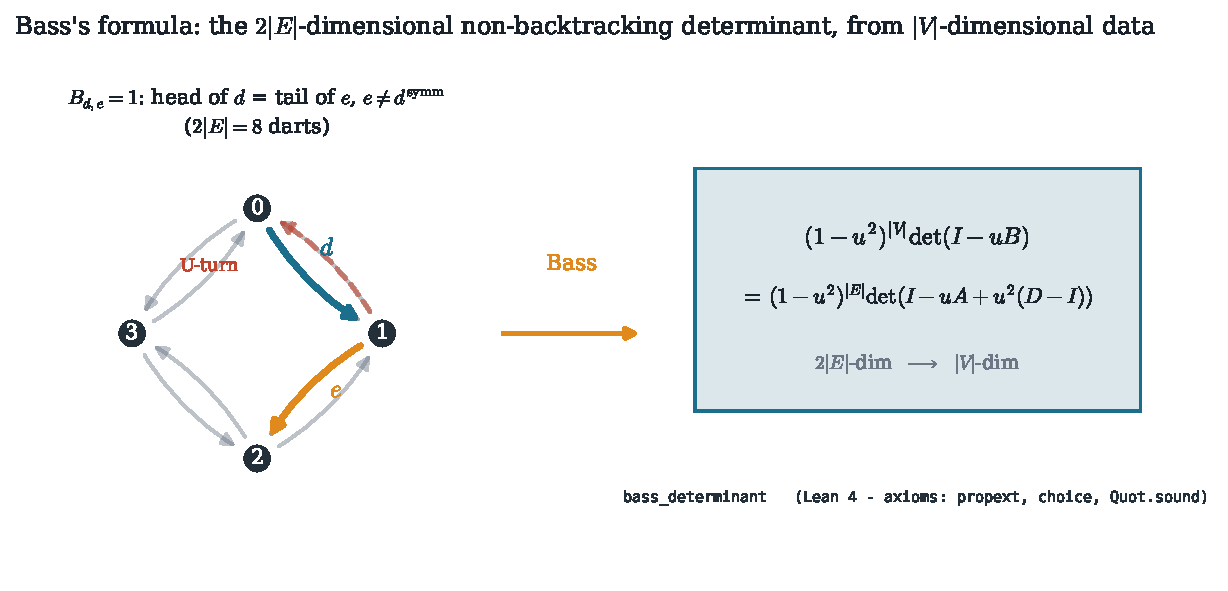
\includegraphics[width=\textwidth]{bass_fig1_nonbacktracking.pdf}
  \caption{La f\'ormula de Bass en un grafo peque\~no. El operador no-retroceso $B$ vive sobre los
  $2|E|$ dardos (izquierda): $B_{d,e}=1$ cuando la cabeza de $d$ es la cola de $e$ y $e$ no es el
  reverso de $d$ (el giro en U, atenuado). Y sin embargo $\det(I-uB)$ se computa con los datos de
  adyacencia/grados de tama\~no $|V|\times|V|$ (derecha). Verificado por m\'aquina como
  \lean{bass\_determinant}.}
  \label{fig:nb}
\end{figure}

% ---------------------------------------------------------------
\section{El resultado}
\label{sec:result}

Basta de mapa; aqu\'i est\'a el territorio. Escribamos $A$ para la matriz de adyacencia, $D$ para la
matriz diagonal de grados, y $B$ para el operador no-retroceso de Hashimoto sobre las $2|E|$ aristas
orientadas (\emph{dardos}). El rec\'iproco de la zeta de Ihara es
$\zeta_G(u)^{-1}=\det(I_{2|E|}-uB)$, y el teorema de Bass lo reduce al tama\~no de los v\'ertices.

\begin{theorem}[F\'ormula del determinante de Bass, en Lean~4]
\label{thm:bass}
Para un grafo finito $G$ sobre un cuerpo, y $u$ en ese cuerpo,
\keyeq{(1-u^2)^{|V|}\,\det\!\bigl(I-uB\bigr)\;=\;(1-u^2)^{|E|}\,\det\!\bigl(I-uA+u^2(D-I)\bigr).}
Equivalentemente $\det(I-uB)=(1-u^2)^{|E|-|V|}\det(I-uA+(D-I)u^2)$. El enunciado es \lean{sorry}-libre;
\lean{\#print axioms SimpleGraph.bass\_determinant} reporta solo \lean{propext},
\lean{Classical.choice}, \lean{Quot.sound}.
\end{theorem}

La Figura~\ref{fig:nb} muestra la reducci\'on; la Tabla~\ref{tab:bass_results} lista cada
ingrediente verificado; la Tabla~\ref{tab:bass_checks} confirma la identidad num\'ericamente.

Un rasgo del enunciado merece una segunda mirada:
\begin{quote}\itshape
  ¿por qu\'e el prefactor $(1-u^2)^{|E|-|V|}$---por qu\'e \emph{esa} potencia, que depende de nada
  m\'as que del n\'umero de aristas y de v\'ertices?
\end{quote}
Porque el exponente es topol\'ogico. Para un grafo conexo $|E|-|V|=\beta_1-1$, donde
$\beta_1=|E|-|V|+1$ es el \emph{primer n\'umero de Betti}---el n\'umero de ciclos independientes, la
dimensi\'on del espacio de ciclos, el rango de $\pi_1(G)$. El prefactor de Bass cuenta los bucles
independientes del grafo; y es exactamente la acumulaci\'on de multiplicidad $|E|-|V|$ de autovalores
$\pm1$ de $B$ que se ve en la Figura~\ref{fig:spectrum}. Una identidad de determinantes conoce en
silencio la topolog\'ia del grafo---lo cual, al fin y al cabo, es lo justo para el rec\'iproco de una
funci\'on que cuenta sus ciclos.

\paragraph{La ruta, en una frase.}
El operador de Hashimoto factoriza como $B=T^{\mathsf T}S-J$, con $S,T$ las matrices de incidencia de
inicio/fin de los dardos y $J$ la involuci\'on de inversi\'on; as\'i $I-uB=(I+uJ)-u\,T^{\mathsf T}S$.
La involuci\'on de inversi\'on tiene un determinante limpio,
\keyeq{\det(I+uJ)\;=\;(1-u^2)^{|E|},}
porque orientar cada arista ordena los $2|E|$ dardos en $|E|$ pares de inversi\'on y convierte $J$ en
una diagonal por bloques de intercambios $2\times2$ (Figura~\ref{fig:reindex}). Sobre un cuerpo con
$1-u^2\neq0$, $I+uJ$ es entonces invertible; factorizarlo de $I-uB$ y aplicar la identidad de
Weinstein--Aronszajn para deslizar $S$ tras $T^{\mathsf T}$ entrega el determinante de tama\~no $|V|$,
y la identidad de incidencia $S(I-uJ)T^{\mathsf T}=A-uD$ lo identifica con el lado derecho.

\paragraph{Contribuciones.} Todo en Lean~4 / Mathlib, todo \lean{sorry}-libre
(Tabla~\ref{tab:bass_results}):
\begin{enumerate}\itemsep2pt
\item \textbf{La f\'ormula del determinante de Bass} (\lean{bass\_determinant}) para todo grafo
  finito sobre un cuerpo, v\'ia la reducci\'on de Sylvester (Secci\'on~\ref{sec:proof}).
\item \textbf{El determinante de la involuci\'on de inversi\'on} $\det(I+uJ)=(1-u^2)^{|E|}$
  (\lean{det\_one\_add\_smul\_reversal}), mediante un reetiquetado por orientaci\'on
  $\Dart\simeq\mathrm{Bool}\times\{\text{dardos positivos}\}$ (\lean{dartEquiv}) que diagonaliza $J$
  por bloques.
\item \textbf{Infraestructura reutilizable}: el operador no-retroceso sobre dardos, la involuci\'on
  de inversi\'on, y el c\'alculo de incidencia de aristas orientadas
  ($S T^{\mathsf T}=A$, $S S^{\mathsf T}=D=T T^{\mathsf T}$, $B=T^{\mathsf T}S-J$, $SJ=T$). Mathlib no
  ten\'ia ninguno.
\end{enumerate}

\paragraph{Qu\'e reclamo como nuevo.} La matem\'atica es cl\'asica (Secci\'on~\ref{sec:related}); la
novedad reside enteramente en la formalizaci\'on. Reclamo, en concreto:
\begin{enumerate}\itemsep1.5pt
\item[(N1)] la primera demostraci\'on verificada por m\'aquina de la que tengo noticia, en cualquier
  asistente de pruebas, de la \emph{f\'ormula del determinante de Bass}, y la primera
  formalizaci\'on del operador no-retroceso (de Hashimoto) y del rec\'iproco de la zeta de Ihara
  $\det(I-uB)$ (basada en b\'usqueda; v\'ease la salvedad abajo);
\item[(N2)] el reetiquetado por orientaci\'on \lean{dartEquiv} y el determinante
  $\det(I+uJ)=(1-u^2)^{|E|}$---una pieza peque\~na y genuinamente reutilizable para cualquier
  argumento que deba orientar las aristas de un grafo;
\item[(N3)] el c\'alculo de incidencia de aristas orientadas como lemas Lean con nombre, incluido un
  lema de conteo de dardos que realiza la matriz de adyacencia como $S T^{\mathsf T}$.
\end{enumerate}
Ninguno de (N1)--(N3) es matem\'atica \emph{nueva} en el sentido de demostraci\'on de teoremas; todos
son contribuciones de \emph{formalizaci\'on}, y los separo del contenido cl\'asico
deliberadamente.

\paragraph{Y, claramente, lo que esto no es.} Es una formalizaci\'on de matem\'atica cl\'asica (Bass,
1992); no demuestra ning\'un teorema nuevo ni lo afirma. Demuestro la identidad de determinantes,
\emph{no} la funci\'on zeta de Ihara anal\'itica (el producto de Euler sobre ciclos primos no est\'a
formalizado). La demuestro \emph{sobre un cuerpo}---el contexto est\'andar, y exactamente lo que el
paso de Sylvester necesita, pues invierte $I+uJ$, una unidad solo cuando $1-u^2\neq0$
(Secci\'on~\ref{sec:field}); la generalidad sobre anillos conmutativos arbitrarios queda mapeada, no
construida. Y ``primera formalizaci\'on'' descansa sobre una b\'usqueda en los tres grandes
ecosistemas de asistentes de pruebas---Lean/Mathlib, el Archive of Formal Proofs (Isabelle) y
Coq/mathcomp---no una auditor\'ia byte a byte de cada biblioteca, as\'i que lo enuncio exactamente
as\'i.

% Tablas (español) para la perla de formalización Ihara--Bass.
% Requiere \usepackage{booktabs,amsmath,amssymb} y \usepackage[table]{xcolor}
% en el preámbulo, más los colores ggteal / ggband definidos allí.

% ---------- Tabla 1: resultados formalizados ----------
\begin{table}[t]
  \centering
  \small
  \arrayrulecolor{ggteal}
  \caption{Los resultados formalizados (Lean~4 / Mathlib). Todos los teoremas son
  \texttt{sorry}-libres; \texttt{\#print axioms} reporta solo \texttt{propext},
  \texttt{Classical.choice}, \texttt{Quot.sound}. El teorema principal es sobre un cuerpo
  (Secci\'on~\ref{sec:field}).}
  \label{tab:bass_results}
  \begin{tabular}{@{}llc@{}}
    \toprule
    \rowcolor{ggteal}
    \textcolor{white}{\textbf{Nombre Lean}} & \textcolor{white}{\textbf{Enunciado}} & \textcolor{white}{\textbf{Estado}} \\
    \midrule
    \rowcolor{ggband}
    \texttt{bass\_determinant} & $(1{-}u^2)^{|V|}\det(I{-}uB)=(1{-}u^2)^{|E|}\det(I{-}uA{+}u^2(D{-}I))$ & demostrado \\
    \texttt{det\_one\_add\_smul\_reversal} & $\det(I+uJ)=(1-u^2)^{|E|}$ & demostrado \\
    \rowcolor{ggband}
    \texttt{dartEquiv} & reetiquetado por orientaci\'on $\mathrm{Dart}\simeq\mathrm{Bool}\times\{\text{dardos pos.}\}$ & definido \\
    \texttt{hashimoto\_eq} & $B=T^{\mathsf T}S-J$ (no-retroceso $=$ contin\'ua $-$ invierte) & demostrado \\
    \rowcolor{ggband}
    \texttt{card\_posDart} & $|\{\text{dardos positivos}\}|=|E|$ (v\'ia apret\'on de manos) & demostrado \\
    \texttt{startInc\_mul\_termInc\_transpose} & $S\,T^{\mathsf T}=A$ (los dardos realizan la adyacencia) & demostrado \\
    \midrule
    \emph{$\zeta_G$ anal\'itica} & producto de Euler sobre ciclos primos & futuro \\
    \rowcolor{ggband}
    \emph{generalidad sobre anillos} & transporte de coeficientes universales desde $\Z[u]$ & futuro \\
    \bottomrule
  \end{tabular}
  \arrayrulecolor{black}
\end{table}

% ---------- Tabla 2: verificaciones numéricas ----------
\begin{table}[t]
  \centering
  \small
  \arrayrulecolor{ggteal}
  \caption{Verificaciones num\'ericas de la f\'ormula de Bass (SymPy, exactas). Para cada grafo, el
  determinante no-retroceso $\det(I-uB)$ se computa directamente sobre los $2|E|$ dardos y se contrasta
  con $(1-u^2)^{|E|-|V|}\det(I-uA+(D-I)u^2)$. Verificado id\'enticamente (tambi\'en para $K_4$, donde
  $|E|-|V|=2$, y el grafo de Petersen; polinomios omitidos por longitud). Los v\'ertices colgantes del
  \emph{bull} aportan factores triviales, as\'i que su determinante solo ve el tri\'angulo.}
  \label{tab:bass_checks}
  \begin{tabular}{@{}lcclc@{}}
    \toprule
    \rowcolor{ggteal}
    \textcolor{white}{\textbf{$G$}} & \textcolor{white}{\textbf{$|V|$}} & \textcolor{white}{\textbf{$|E|$}} & \textcolor{white}{\textbf{$\det(I-uB)$}} & \textcolor{white}{\textbf{¿Bass?}} \\
    \midrule
    \rowcolor{ggband}
    $K_3$  & $3$ & $3$ & $(u^{3}-1)^{2}$ & $\checkmark$ \\
    $C_4$  & $4$ & $4$ & $(u^{4}-1)^{2}$ & $\checkmark$ \\
    \rowcolor{ggband}
    $C_5$  & $5$ & $5$ & $(u^{5}-1)^{2}$ & $\checkmark$ \\
    \emph{bull} & $5$ & $5$ & $(u^{3}-1)^{2}$ & $\checkmark$ \\
    \rowcolor{ggband}
    $K_4$  & $4$ & $6$ & grado $12$, $|E|-|V|=2$ (ver fuente) & $\checkmark$ \\
    \bottomrule
  \end{tabular}
  \arrayrulecolor{black}
\end{table}


% ---------------------------------------------------------------
\section{¿Qu\'e son exactamente los objetos?}
\label{sec:setting}

Una pregunta precede a las definiciones:
\begin{quote}\itshape
  de todos los operadores que se podr\'ian colgar de las aristas de un grafo, ¿por qu\'e \emph{este}
  ---por qu\'e prohibir el \'unico movimiento de dar marcha atr\'as de inmediato?
\end{quote}
Porque el retroceso inunda un camino de retornos triviales. En cualquier grafo, la contribuci\'on
dominante a $\operatorname{tr}(A^k)$ viene de caminos que se alejan y desandan sus pasos---los mismos
retornos que un \'arbol ya tiene, la sombra \'arbol de la Secci\'on~\ref{sec:trace}. Quita los giros
en U y solo sobrevive el contenido de ciclo genuino: el espectro del operador no-retroceso ve los
bucles del grafo, no su sombra \'arbol, y su mayor autovalor mide la ramificaci\'on verdadera. Por
eso el \emph{mismo} operador que define la zeta de Ihara fija tambi\'en el umbral de percolaci\'on de
una red---ambos preguntan, en el fondo, con qu\'e rapidez proliferan los caminos que no se
desandan. Con ese motivo en mano, hay que fijar los operadores.

Trabajo sobre un tipo de v\'ertices finito $V$ con adyacencia decidible. Mathlib ya tiene el tipo
\lean{SimpleGraph.Dart} de aristas \emph{orientadas}; la inversi\'on $d\mapsto d^{\mathrm{symm}}$ es
una involuci\'on sin puntos fijos sobre los $2|E|$ dardos, y esa involuci\'on es toda la raz\'on de
que la f\'ormula tenga la forma que tiene.

\begin{definition}[Los cuatro operadores]
Sobre un anillo conmutativo $R$: la \emph{matriz de grados}
$D=\operatorname{diagonal}(v\mapsto\deg v)$; la matriz de permutaci\'on de \emph{inversi\'on} $J$, con
$J_{d,e}=[\,e=d^{\mathrm{symm}}\,]$; el operador \emph{no-retroceso} (de Hashimoto) $B$, con
$B_{d,e}=[\,d.\mathrm{snd}=e.\mathrm{fst}\ \wedge\ e\neq d^{\mathrm{symm}}\,]$; y las matrices de
incidencia de inicio/fin $S,T\colon V\times\Dart$, con $S_{v,d}=[\,d.\mathrm{fst}=v\,]$,
$T_{v,d}=[\,d.\mathrm{snd}=v\,]$.
\end{definition}

Con $A$ la matriz de adyacencia de Mathlib, el teorema demostrado es la identidad enmarcada del
Teorema~\ref{thm:bass}, enunciada en Lean sobre un cuerpo. Mathlib tiene una rica teor\'ia de grafos
simples, dardos y determinantes, pero ning\'un operador no-retroceso ni zeta de Ihara; construir el
operador y su c\'alculo de incidencia fue un prerrequisito, y no pude hallar formalizaci\'on previa de
la f\'ormula de Bass---ni del determinante del operador de Hashimoto---en ning\'un asistente.\footnote{B\'usqueda
razonable (no exhaustiva) en Lean/Mathlib, el Archive of Formal Proofs (Isabelle) y el ecosistema
Coq/MathComp (junio de 2026): aparecen la adyacencia de grafos, los polinomios caracter\'isticos y el
polinomio de emparejamientos (en mi propio trabajo anterior), pero no hall\'e formalizaci\'on de la
zeta de Ihara, la f\'ormula de Bass o el operador no-retroceso. De ah\'i ``que yo sepa''.}

% ---------------------------------------------------------------
\section{C\'omo una m\'aquina reduce $2|E|$ a $|V|$}
\label{sec:proof}

Antes de cualquier t\'actica, una pregunta en la que vale la pena detenerse:
\begin{quote}\itshape
  ¿por qu\'e un determinante sobre $2|E|$ aristas habr\'ia de ser en secreto un determinante sobre
  $|V|$ v\'ertices---qu\'e hace que el objeto mayor colapse?
\end{quote}
La respuesta est\'a escondida en la \emph{forma} de $B$, y es el coraz\'on conceptual de toda la
f\'ormula. El operador de Hashimoto no es arbitrario: se parte como $B=T^{\mathsf T}S-J$, una parte
$T^{\mathsf T}S$ que \emph{factoriza por los v\'ertices}---tiene rango a lo sumo $|V|$, pues $S$ y $T$
pasan por el espacio de v\'ertices de dimensi\'on $|V|$---m\'as la involuci\'on de inversi\'on $J$. La
parte que factoriza por v\'ertices es exactamente lo que una identidad de Sylvester puede bajar a
tama\~no $|V|$; la involuci\'on $J$ es exactamente lo que las potencias de $(1-u^2)$ absorben. As\'i
que el colapso no es un milagro: es la afirmaci\'on de que el operador de aristas porta solo tanta
informaci\'on espectral genuina como $|V|$ v\'ertices, envuelta en una involuci\'on. La f\'ormula de Bass es
la contabilidad precisa de esa partici\'on, y la demostraci\'on de abajo es esa contabilidad hecha
expl\'icita. El argumento cl\'asico factoriza el determinante grande invirtiendo $I+uJ$ y deslizando
las matrices de incidencia una sobre otra; convertirlo en una demostraci\'on verificada signific\'o
hacer expl\'icito cada ``obs\'ervese que'', en tres movimientos.

\paragraph{El c\'alculo de incidencia.}
Todo descansa sobre cuatro identidades, cada una una suma finita sobre dardos (todas pre-verificadas
num\'ericamente antes de formalizar):
\keyeq{S\,T^{\mathsf T}=A,\qquad S\,S^{\mathsf T}=D=T\,T^{\mathsf T},\qquad
  B=T^{\mathsf T}S-J,\qquad S\,J=T.}
La primera dice que los dardos de $v$ a $w$ realizan la matriz de adyacencia (un lema de conteo de
dardos, \lean{adj\_dart\_card}); la tercera es la definici\'on de ``no-retroceso'' como ``contin\'ua,
menos invierte''; la cuarta dice que la inversi\'on intercambia los dos extremos de un dardo. De
$SJ=T$ junto con $J^{\mathsf T}=J$ y $J^2=I$ se obtiene la compa\~nera $T\,T^{\mathsf T}=D$ gratis,
reusando $S\,S^{\mathsf T}=D$ en vez de recontar.

\paragraph{El determinante de la involuci\'on de inversi\'on.}
El c\'alculo que sostiene el peso es $\det(I+uJ)=(1-u^2)^{|E|}$. He aqu\'i la idea, y el \'unico lugar
donde entra una elecci\'on real. Fija cualquier orden lineal en $V$; llama \emph{positivo} a un dardo
cuando su cola precede a su cabeza. Cada arista tiene exactamente un dardo positivo, y la inversi\'on
de un dardo no positivo es positiva. Esto produce una equivalencia (\lean{dartEquiv},
Figura~\ref{fig:reindex})
\keyeq{\Dart\;\simeq\;\mathrm{Bool}\times\{\text{dardos positivos}\},}
bajo la cual $J$---que solo intercambia cada dardo con su reverso---se vuelve una \emph{diagonal por
bloques} del intercambio $2\times2$, un bloque por arista. As\'i $I+uJ$ se vuelve una diagonal por
bloques de $\bigl(\begin{smallmatrix}1&u\\u&1\end{smallmatrix}\bigr)$, y como los dardos positivos
biyectan con las aristas ($|\{\text{dardos positivos}\}|=|E|$, por el lema del apret\'on de manos;
\lean{card\_posDart}), \lean{Matrix.det\_blockDiagonal} de Mathlib da $\det(I+uJ)=(1-u^2)^{|E|}$,
aportando cada bloque $1-u^2$.

\begin{figure}[t]
  \centering
  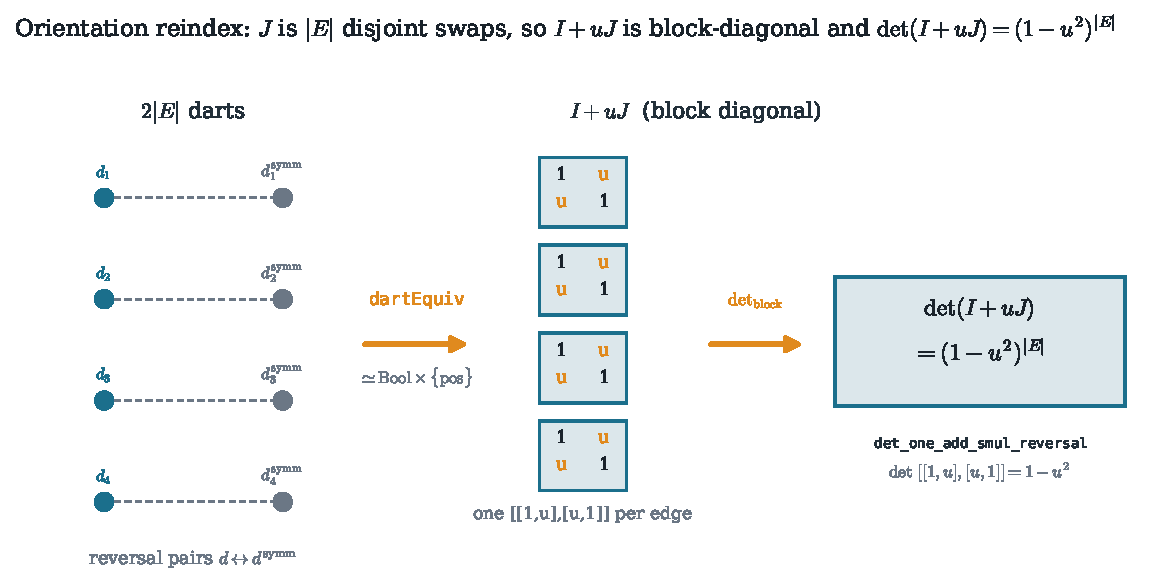
\includegraphics[width=\textwidth]{bass_fig2_reindex.pdf}
  \caption{El reetiquetado por orientaci\'on \lean{dartEquiv}: elegir una direcci\'on por arista
  ordena los $2|E|$ dardos en $|E|$ pares de inversi\'on, diagonalizando $J$ por bloques. Entonces
  $I+uJ$ es una diagonal por bloques de $\bigl(\begin{smallmatrix}1&u\\u&1\end{smallmatrix}\bigr)$,
  de modo que $\det(I+uJ)=(1-u^2)^{|E|}$ (\lean{det\_one\_add\_smul\_reversal}).}
  \label{fig:reindex}
\end{figure}

\paragraph{La reducci\'on de Sylvester.}
Como $B=T^{\mathsf T}S-J$, tenemos $I-uB=(I+uJ)-u\,T^{\mathsf T}S$. Sobre un cuerpo con $1-u^2\neq0$,
el paso anterior hace $I+uJ$ \emph{invertible}, con $(I+uJ)^{-1}=(1-u^2)^{-1}(I-uJ)$ (inmediato de
$(I+uJ)(I-uJ)=(1-u^2)I$). Factorizarlo y aplicar la identidad de Weinstein--Aronszajn
\lean{Matrix.det\_one\_sub\_mul\_comm} para deslizar $S$ tras $T^{\mathsf T}$ da el determinante de
tama\~no $|V|$
\[
  \det(I-uB)=(1-u^2)^{|E|}\det\!\bigl(I-u\,S(I+uJ)^{-1}T^{\mathsf T}\bigr),
\]
y la identidad de incidencia $S(I-uJ)T^{\mathsf T}=A-uD$ colapsa el factor derecho a
$(1-u^2)^{-|V|}\det(I-uA+u^2(D-I))$. Despejar denominadores es el teorema. El valor degenerado
$u^2=1$, donde $I+uJ$ es singular, se trata aparte: ah\'i el enunciado se reduce a los casos sin
aristas y de grafo vac\'io, donde ambos lados se anulan o son trivialmente iguales.

% ---------------------------------------------------------------
\section{De d\'onde viene la hip\'otesis de cuerpo}
\label{sec:field}

Ser\'ia f\'acil enunciar el teorema sobre un anillo conmutativo arbitrario y confiar en silencio; no
lo hago. La reducci\'on de Sylvester \emph{invierte} $I+uJ$ y \emph{divide} por $1-u^2$, ambas
leg\'itimas solo cuando $1-u^2$ es una unidad---es decir, sobre un cuerpo, lejos de $u^2=1$. Este es
el contexto est\'andar de la f\'ormula de Bass (se trabaja sobre $\mathbb{C}$), y es honesto decirlo
en vez de vestir la demostraci\'on con m\'as generalidad de la que tiene.

La raz\'on de que la brecha sea real, no cosm\'etica: las manipulaciones sin inversa por s\'i solas
---multiplicar por $I-uJ$, usar $\det(I-uJ)=(1-u^2)^{|E|}$ y Weinstein--Aronszajn en $t=1$---entregan
la identidad \emph{multiplicada por un $(1-u^2)^{|E|}$ extra}, y recuperar el enunciado ajustado
exige cancelar ese factor, lo que un cuerpo permite y un anillo con divisores de cero no. La
generalidad plena sobre anillos conmutativos se sigue, no obstante, por un transporte de
coeficientes universales: demostrar la identidad sobre $\Z[u]$, donde $1-u^2$ no es divisor de cero y
la cancelaci\'on es legal, y luego cambiar de base por cualquier morfismo de anillos $\Z[u]\to R,\
u\mapsto u$, usando que los determinantes conmutan con homomorfismos de anillos. Describo esta ruta
pero no la recorro; la versi\'on sobre cuerpo es la verificada por m\'aquina, y no reclamo m\'as.

% ---------------------------------------------------------------
\section{Dos lados de una misma f\'ormula de traza}
\label{sec:trace}

¿Qu\'e tiene que ver el lado Ihara con el polinomio de emparejamientos de los art\'iculos~I y~II~\cite{PartI,PartII}?
Son las dos mitades de una sola contabilidad de caminos cerrados. Esquem\'aticamente, la traza de una
potencia de la matriz de adyacencia se parte en una parte \emph{tipo \'arbol} y una parte
\emph{c\'iclica},
\keyeq{\operatorname{tr}(A^k)\;=\;\underbrace{p_k}_{\text{polinomio de emparej. / \'arbol}}
  \;+\;\underbrace{N_k}_{\text{no-retroceso / ciclos}},}
con la misma banda $2\sqrt{\Delta-1}$ gobernando ambos lados (Figura~\ref{fig:trace}). El polinomio
de emparejamientos es la sombra del recubrimiento universal (\'arbol) del conteo de caminos; el
determinante de Ihara--Bass cuenta los ciclos genuinos, organizados por el grupo fundamental $\pi_1$.

He aqu\'i una pregunta que vale la pena llevarse de este art\'iculo:
\begin{quote}\itshape
  ¿por qu\'e el \emph{mismo} n\'umero, $2\sqrt{\Delta-1}$, acota las ra\'ices del polinomio de
  emparejamientos (Paper~II) y marca la recta cr\'itica de la zeta de Ihara---dos objetos
  construidos a partir de $G$ de formas en apariencia inconexas?
\end{quote}
Porque ambos son sombras de un mismo objeto: el \'arbol $\Delta$-regular que recubre universalmente a
$G$. Su radio espectral es exactamente $2\sqrt{\Delta-1}$ (Kesten, 1959). El polinomio de
emparejamientos ve ese n\'umero como el borde de la medida de Plancherel (Kesten--McKay) del \'arbol;
la zeta de Ihara lo ve como la recta cr\'itica de una hip\'otesis de Riemann para grafos. Un \'arbol,
dos sombras, un n\'umero---y una raz\'on para sospechar que la f\'ormula de traza de arriba es
precisamente el enunciado que hace que la coincidencia deje de serlo. Con el lado \'arbol formalizado
en los art\'iculos anteriores y el lado ciclo aqu\'i, ambos extremos de ese puente existen ya en
Lean, y la f\'ormula de traza misma ($p_k=\operatorname{tr}(A^k)-N_k$, exacta hasta la cintura) se
vuelve un objetivo bien planteado.

\begin{figure}[t]
  \centering
  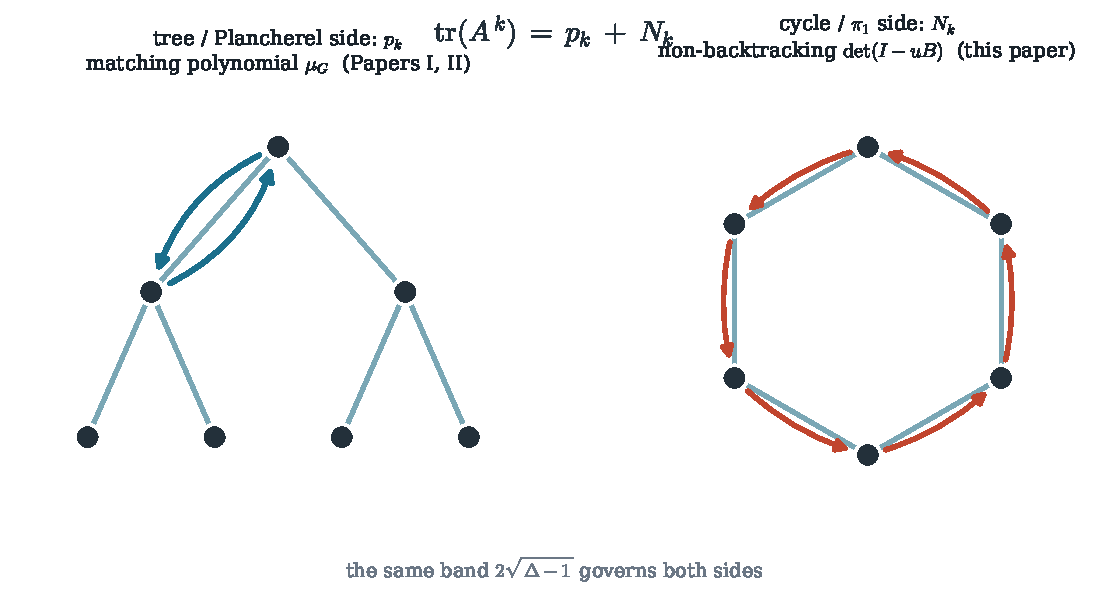
\includegraphics[width=0.92\textwidth]{bass_fig5_trace.pdf}
  \caption{Dos lados de una misma contabilidad de caminos cerrados. La parte \'arbol (Plancherel)
  $p_k$ es el polinomio de emparejamientos---el conteo de caminos en el recubrimiento universal,
  donde todo retorno es un retroceso (art\'iculos~I y~II); la parte ciclo ($\pi_1$) $N_k$ es el
  conteo no-retroceso $\det(I-uB)$ de este art\'iculo. La misma banda $2\sqrt{\Delta-1}$ confina
  ambos. Con ambos extremos ya en Lean, la f\'ormula de traza $p_k=\operatorname{tr}(A^k)-N_k$ se
  vuelve un objetivo bien planteado.}
  \label{fig:trace}
\end{figure}

Un primer dividendo es ya visible. El prefactor $(1-u^2)^{|E|-|V|}$ de Bass es exactamente la fuente
de un rasgo llamativo del espectro no-retroceso: una acumulaci\'on de multiplicidad $|E|-|V|$ de
autovalores en $\pm1$, con los autovalores ``ciclo'' restantes llenando un disco cuyo radio lo fija
la varianza de los grados, no la media (Figura~\ref{fig:spectrum})---el mismo disco cuyo borde real
da el umbral de percolaci\'on.

\begin{figure}[t]
  \centering
  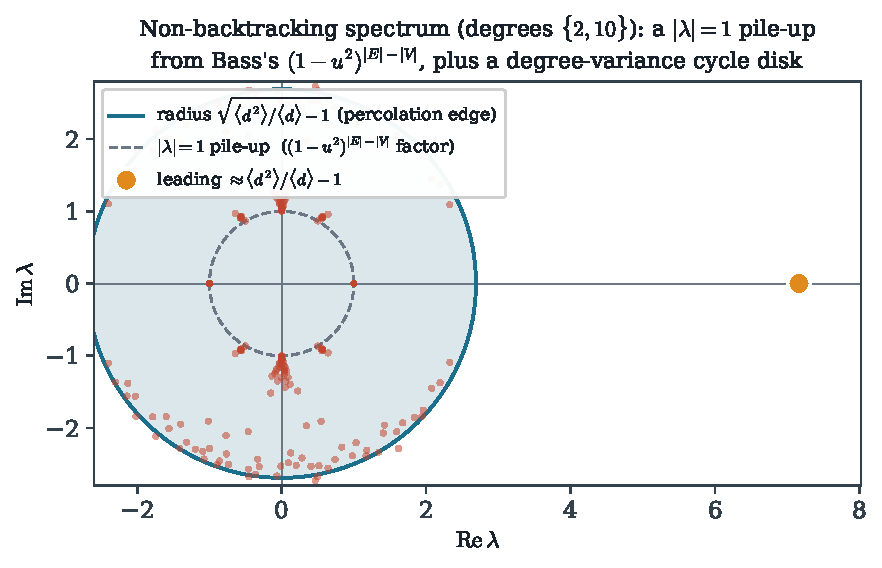
\includegraphics[width=0.9\textwidth]{bass_fig3_spectrum.pdf}
  \caption{El espectro no-retroceso de un grafo de grado irregular (modelo de configuraci\'on, grados
  $2$ y $10$). Una gran multiplicidad se sit\'ua sobre el c\'irculo unidad---los autovalores $\pm1$
  forzados por el factor $(1-u^2)^{|E|-|V|}$ de Bass---mientras que los autovalores ``ciclo'' llenan
  un disco de radio $\sqrt{\langle d^2\rangle/\langle d\rangle-1}$ (varianza de grados, no media),
  cuyo borde real es el umbral de percolaci\'on. Calculado; la estructura la explica
  \lean{bass\_determinant}.}
  \label{fig:spectrum}
\end{figure}

% ---------------------------------------------------------------
\section{Implicaciones}
\label{sec:implications}

Tres tipos de implicaci\'on, en orden decreciente de cu\'an firmemente puedo afirmarlas, y un
apunte metodol\'ogico.

\paragraph{Piezas certificadas y reutilizables.}
El operador no-retroceso, el c\'alculo de incidencia de aristas orientadas, el determinante de la
involuci\'on $\det(I+uJ)=(1-u^2)^{|E|}$ y el reetiquetado por orientaci\'on est\'an ahora verificados
por m\'aquina y disponibles para quien formalice teor\'ia espectral de grafos, mezcla de expansores o
funciones zeta de grafos; Mathlib no ten\'ia ninguno. El reetiquetado
$\Dart\simeq\mathrm{Bool}\times\{\text{dardos positivos}\}$ es en particular una pieza peque\~na pero
genuinamente reutilizable para cualquier argumento que necesite orientar aristas. Esta es la
implicaci\'on que puedo afirmar con m\'as firmeza.

\paragraph{Un punto de apoyo para la f\'ormula de traza y m\'as all\'a.}
Con los lados \'arbol (polinomio de emparejamientos) y ciclo (Ihara--Bass) ya formalizados, la
f\'ormula de traza de grafos que los une es ahora un objetivo concreto, igual que la zeta de Ihara
anal\'itica---el producto de Euler sobre ciclos primos del que este determinante es rec\'iproco. Si
esos hitos se construyen, estos son cimientos sobre los que pueden apoyarse.

\paragraph{La matem\'atica, con una nota de cautela.}
Los espectros no-retroceso sustentan umbrales finos de epidemia y percolaci\'on, la detecci\'on
espectral de comunidades y el an\'alisis de expansores---por eso importa la identidad subyacente. Soy
cauto, no obstante, con tomar prestada esa importancia para este art\'iculo: formalizar una identidad
de determinantes fundacional no env\'ia por s\'i misma un algoritmo ni una red. Su valor reside en
cimientos certificados y en el corpus creciente de matem\'atica formalizada, no en aplicaci\'on
inmediata; reclamo lo primero, no lo segundo.

\paragraph{Un apunte metodol\'ogico.}
Este desarrollo se realiz\'o con un sistema de IA como instrumento de investigaci\'on: propuso
definiciones, lemas y t\'acticas, y un bucle de compilaci\'on-como-or\'aculo verific\'o o rechaz\'o
cada uno contra el n\'ucleo. La contabilidad cuidadosa de este art\'iculo---cada afirmaci\'on
dimensionada a exactamente lo demostrado, la hip\'otesis de cuerpo enunciada con la misma claridad que
el resultado---es parte de lo que espero que el trabajo ilustre: que la formalizaci\'on asistida por
IA puede resistir la sobreafirmaci\'on que el m\'etodo invita, precisamente porque el asistente de
pruebas, y no el asistente, tiene la \'ultima palabra.

% ---------------------------------------------------------------
\section{D\'onde esto deja de ser \'util}
\label{sec:context}

La honestidad corta por ambos lados, as\'i que enuncio los l\'imites con la misma claridad que el
resultado. El teorema es una \emph{identidad de determinantes}, no la funci\'on zeta anal\'itica; por
s\'i mismo no dice nada sobre la ubicaci\'on de los polos de la zeta ni sobre los conteos de ciclos
primos que lo motivan---eso requiere el producto de Euler que no formalic\'e. Est\'a demostrado
\emph{sobre un cuerpo}; quien necesite la f\'ormula de Bass sobre $\Z$ o un anillo conmutativo
arbitrario debe aceptar el argumento de coeficientes universales de la Secci\'on~\ref{sec:field} en
confianza o formalizarlo. Y es una \emph{sola identidad}, no una teor\'ia: la caracterizaci\'on
hip\'otesis-de-Riemann-para-grafos de los grafos de Ramanujan, las refinaciones de la zeta de aristas
y multivariable, y la conexi\'on con el Bethe--Hessian y con la propagaci\'on de creencias est\'an
todas r\'io abajo, y todas a\'un sin formalizar. Este art\'iculo es una piedra certificada en ese
camino, y prefiero nombrar el camino que exagerar la piedra.

% ---------------------------------------------------------------
\section{Trabajo relacionado}
\label{sec:related}

La matem\'atica es cl\'asica: la funci\'on zeta de Ihara~\cite{Ihara1966}, el operador de aristas de
Hashimoto~\cite{Hashimoto1989}, la f\'ormula del determinante de Bass~\cite{Bass1992}, el relato
moderno de Terras~\cite{Terras2011}, y las demostraciones elementales de Kotani--Sunada y
otros~\cite{KotaniSunada2000}; el papel del espectro no-retroceso en ciencia de redes es
reciente~\cite{KarrerNewmanZdeborova2014}. En el lado de la formalizaci\'on, Mathlib~\cite{Mathlib2020}
aporta grafos simples, dardos y determinantes pero ni el operador no-retroceso ni la zeta de Ihara.
Este desarrollo es el ``lado Ihara'', complementario de mis formalizaciones previas en Lean del polinomio
de emparejamientos~\cite{PartI,PartII}; no tengo noticia de ning\'un tratamiento verificado por
m\'aquina previo de la f\'ormula de Bass, la zeta de Ihara o el operador de Hashimoto en ning\'un
asistente de pruebas.

% ---------------------------------------------------------------
\section{Conclusi\'on}

Part\'i de una pregunta simple---¿puede el determinante no-retroceso de dimensi\'on $2|E|$ computarse
a partir de datos de dimensi\'on $|V|$?---y la segu\'i, en un asistente de pruebas, hasta la respuesta
completa y verificada de Bass. Nada de esto es matem\'atica nueva; la contribuci\'on es que la
identidad de Ihara--Bass, el operador no-retroceso y el determinante de la involuci\'on de inversi\'on
est\'an ahora verificados por m\'aquina donde no pude hallar formalizaci\'on previa, y que el lado
ciclo de la f\'ormula de traza emparejamientos/Ihara convive ya con el lado \'arbol en la misma
biblioteca. La funci\'on zeta anal\'itica y la generalidad plena sobre anillos quedan por delante,
mapeadas pero no construidas. Lo ofrezco como una perla y una invitaci\'on.

\paragraph{Artefactos.} Todas las fuentes Lean (\lean{sorry}-libres, dependientes solo de los tres
axiomas est\'andar; v\'ease la Tabla~\ref{tab:bass_results}), las figuras y las verificaciones
num\'ericas de la Tabla~\ref{tab:bass_checks} est\'an en
\begin{center}
\url{https://github.com/karlesmarin/godsil-gutman-lean}\quad(\lean{Ihara/Bass.lean}).
\end{center}
Verifica la huella de axiomas con \lean{\#print axioms SimpleGraph.bass\_determinant}
$\rightsquigarrow$ \lean{[propext, Classical.choice, Quot.sound]}.

\bibliographystyle{plain}
\bibliography{references}

\end{document}
